\documentclass[11pt]{article}
\usepackage[utf8]{inputenc}
\usepackage[T1]{fontenc}
\usepackage{geometry}
\geometry{a4paper, margin=25mm}
\usepackage{graphicx}
\usepackage{booktabs}
\usepackage{amsmath}
\usepackage{natbib}
\usepackage{hyperref}
\usepackage{xcolor}
\newcommand{\FishNtcPAuto}{0.078}
\newcommand{\FishNtcPRingZero}{0.171}
\newcommand{\FishNtcPRingOne}{0.079}
\newcommand{\FishNtcPRingTwo}{0.067}
\newcommand{\FishNtcQAuto}{0.018}
\newcommand{\FishNtcQSpill}{0.043}
\newcommand{\FishAutoHits}{968}
\newcommand{\FishSpillHits}{2,249}
\newcommand{\FishAutoFdp}{0.32}
\newcommand{\FishSpillFdp}{0.53}
\newcommand{\FishNTests}{51,000}
\newcommand{\FishArtifactFrac}{0.005}
\newcommand{\FishAlphaRingZero}{0.389}
\newcommand{\FishArtifactTargets}{34}
\newcommand{\FishPredRepAuto}{0.09}
\newcommand{\FishPredNullRepAuto}{0.11}
\newcommand{\FishPredRepSpill}{0.23}
\newcommand{\FishPredNullRepSpill}{0.24}
\newcommand{\FishPredGoAuto}{0.09}
\newcommand{\FishPredNullGoAuto}{0.10}
\newcommand{\FishPredGoSpill}{0.21}
\newcommand{\FishPredNullGoSpill}{0.22}
\newcommand{\FishTopTarget}{MAP3K7}
\newcommand{\FishTopScore}{2.50}
\newcommand{\FishNtcScoreQ}{0.22}
\newcommand{\FishNAboveNtc}{31}
\newcommand{\FishNRanked}{31}
\newcommand{\MultiNtcPAuto}{0.063}
\newcommand{\MultiNtcPRingZero}{n/a}
\newcommand{\MultiNtcPRingOne}{n/a}
\newcommand{\MultiNtcPRingTwo}{0.096}
\newcommand{\MultiNtcQAuto}{0.016}
\newcommand{\MultiNtcQSpill}{0.022}
\newcommand{\MultiAutoHits}{223}
\newcommand{\MultiSpillHits}{667}
\newcommand{\MultiAutoFdp}{1.00}
\newcommand{\MultiSpillFdp}{0.62}
\newcommand{\MultiNTests}{70,015}
\newcommand{\MultiArtifactFrac}{-0.056}
\newcommand{\MultiAlphaRingZero}{-0.406}
\newcommand{\MultiArtifactTargets}{219}
\newcommand{\MultiPredRepAuto}{0.09}
\newcommand{\MultiPredNullRepAuto}{0.10}
\newcommand{\MultiPredRepSpill}{0.01}
\newcommand{\MultiPredNullRepSpill}{0.02}
\newcommand{\MultiPredGoAuto}{0.08}
\newcommand{\MultiPredNullGoAuto}{0.08}
\newcommand{\MultiPredGoSpill}{0.01}
\newcommand{\MultiPredNullGoSpill}{0.02}
\newcommand{\MultiTopTarget}{Ube2f}
\newcommand{\MultiTopScore}{23.59}
\newcommand{\MultiNtcScoreQ}{22.69}
\newcommand{\MultiNAboveNtc}{1}
\newcommand{\MultiNRanked}{187}
\newcommand{\HeldoutRho}{0.06}
\newcommand{\HeldoutNull}{0.04}
\newcommand{\HeldoutP}{0.11}
\newcommand{\HeldoutOverlap}{0}
\newcommand{\FishClonRatio}{15}
\newcommand{\FishClonZ}{56}
\newcommand{\FishMisCor}{0.72}
\newcommand{\MultiClonRatio}{137}
\newcommand{\MultiClonZ}{1682}
\newcommand{\MultiMisCor}{0.71}
\newcommand{\MapClonRatio}{2}
\newcommand{\MapClonZ}{38}
\newcommand{\MapMisCor}{n/a}
\newcommand{\DbitClonRatio}{1}
\newcommand{\DbitClonZ}{25}
\newcommand{\DbitMisCor}{0.99}
\newcommand{\StereoClonRatio}{8}
\newcommand{\StereoClonZ}{31}
\newcommand{\StereoMisCor}{0.17}


\title{Calibrated estimation of cell-autonomous and spillover effects in spatial CRISPR screens: clonal structure, local nulls and what survives them}
\author{Matin Gerami\\ Universit\'e d'\'Evry Paris-Saclay}
\date{Draft, \today}

\begin{document}
\maketitle

\begin{abstract}
Spatial CRISPR screens promise to separate what a perturbation does to the perturbed cell
(cell-autonomous effect) from what it does to its neighbours (spillover). Published analyses
report intercellular effects with ad hoc statistics that compare control cells with and
without perturbed neighbours. We formalise spillover as an estimand under network
interference with explicit, testable assumptions, build a ground-truth simulator with planted
autonomous, spillover, bleed-through, density, batch, clonal and misassignment effects, and
benchmark a ladder of estimators against space-blind and ad hoc baselines on five public
screens spanning four technologies (MERFISH-based Perturb-FISH and Perturb-Multi, microfluidic
Perturb-DBiT, Visium-based Perturb-map, Stereo-seq Spatial Perturb-seq). Three findings
organise the results. First, in every in vivo screen, cells carrying the same guide are
spatially clustered far beyond a stratified permutation null (\FishClonRatio x in Perturb-FISH,
\MultiClonRatio x in Perturb-Multi on adjacent pairs), and unlabelled neighbours of perturbed
cells carry the perturbed expression signature (median $r$ = \FishMisCor{} and \MultiMisCor),
so a missing guide call is not evidence of an unperturbed cell; recipients of spillover must
carry a confirmed non-target guide. Second, the standard stratified permutation null and heteroskedasticity-robust regression
standard errors are both anticonservative because exposed recipients share the niche of one
clone; non-targeting pseudo-targets, run through every estimator as mandatory calibration,
exceed the nominal false-positive rate (\EOneGlobalNtcPRingZero{} at the first ring in Perturb-FISH,
\MultiEOneNtcP{} in Perturb-Multi). Local spatial tiles as strata restore calibration
(\EOneTileNtcP{} at $p<0.05$) but identify only \EOneTileNTests{} of \EOneGlobalNTests{} tests, and
with them no autonomous (\EOneTileAutoHits) and \EOneTileSpillHits{} spillover calls survive: in a
clonal screen even the "autonomous" contrast of a clone against distant controls is a niche
contrast. Regression adjustment with a spatial basis, with or without a permutation null,
fails the pre-registered calibration gate on the simulator under clonal assignment with
analytic standard errors (outer-ring false positives 0.14 to 0.29); with a stratified
permutation null its non-targeting rates on Perturb-FISH are nominal at every ring
(\FishNtcPAuto, \FishNtcPRingZero, \FishNtcPRingOne, \FishNtcPRingTwo) and its calls collapse
to \FishAutoHits{} autonomous and \FishSpillHits{} spillover at $q<0.1$ (non-targeting
expectation about 8 and 0), with a minor bleed-through component (first-ring variance
explained minus last ring \FishArtifactFrac) and a hypothesis ranking led by \FishTopTarget. Third, the published
neighbour $t$-test design has false discovery proportions of 0.3 to 0.6 on the simulator, and a
graph neural network ranks planted spillover well (AUROC about 0.9) with unusable intervals.
Gene embeddings (Perturb-seq, GO, ESM2) do not predict held-out spillover profiles
beyond a permuted-embedding null, and nothing transfers across technologies (Spearman
\HeldoutRho, null \HeldoutNull). We release \texttt{spatialspill}, the simulator, loaders for
all five datasets and a lab notebook with pre-registrations and amendments.
\end{abstract}

\section{Introduction}
\label{sec:intro}
Pooled CRISPR screens read out by imaging or spatial sequencing place each perturbed cell in
its tissue context \citep{binan2025,saunders2025,baysoy2026,dhainaut2022,shen2026}. This
makes a new kind of effect measurable: the change in an unperturbed cell caused by a
perturbed neighbour. Perturb-FISH reported such intercellular effects in vitro and in
tumours \citep{binan2025}; Perturb-map used lesion-level labels to associate knockouts with
immune infiltration \citep{dhainaut2022}. These analyses treat the neighbour effect as a
difference between control cells with and without a perturbed neighbour, without a causal
estimand, without a null that respects geometry, and without separating true intercellular
signalling from segmentation bleed-through, density, batch, tissue edge and clonal structure.

We ask which intercellular effects in public spatial screens survive a formal treatment of
interference, mandatory non-targeting calibration, and explicit artifact modelling. The
answer is sobering and, we argue, useful: the dominant structure in every in vivo dataset is
clonal or delivery-driven clustering of same-guide cells, which confounds both autonomous and
spillover estimates unless the null is local; once it is, one dataset retains a modest,
calibrated spillover signal and the other does not.

\section{Results}
\label{sec:results}

\subsection{Estimands and identification}
Section~\ref{sec:methods} and \texttt{docs/estimands.md} define the autonomous effect
$\tau_g(c)$ and the spillover $\tau_g(b,c)$ at distance ring $b$ on recipient type $c$ under
partial interference across samples \citep{hudgens2008} and a local exposure mapping
\citep{aronow2017}. Identification needs ignorable assignment within strata (A3), no
unmeasured spatial confounding beyond covariates (A4) and positivity (A5). A4 is untestable
in general but has a testable implication: non-targeting guides, treated as pseudo-targets,
must yield null autonomous and spillover estimates at the nominal rate. Every analysis below
reports this check.

\subsection{Same-guide cells cluster in every in vivo screen}
Figure~\ref{fig:clonality} summarises the audit. On the pruned Delaunay graph, pairs of
adjacent cells sharing a target are \FishClonRatio{} times more frequent than under the
stratified permutation null in Perturb-FISH ($z$ = \FishClonZ), \MultiClonRatio{} times in
Perturb-Multi ($z$ = \MultiClonZ), with Perturb-map lesions (by construction), Perturb-DBiT
pixels and Spatial Perturb-seq showing the same pattern at lower magnitude. The excess is
guide-specific (same-target-other-guide pairs are not enriched) and, in Perturb-FISH, flat
over 0 to 100~$\mu$m, the signature of clonal growth of transduced tumour cells rather than of
first-ring barcode misassignment. Unassigned cells adjacent to cells of target $g$ are shifted
towards $g$'s autonomous profile (median correlation \FishMisCor{} over 30 targets in
Perturb-FISH, \MultiMisCor{} over 60 in Perturb-Multi). With guide-call rates of 4 to 5\%,
most unassigned neighbours of a perturbed cell are undetected siblings. Spillover recipients
and controls must therefore carry a confirmed guide other than $g$ (non-targeting by default).

\begin{figure}[t]
\centering
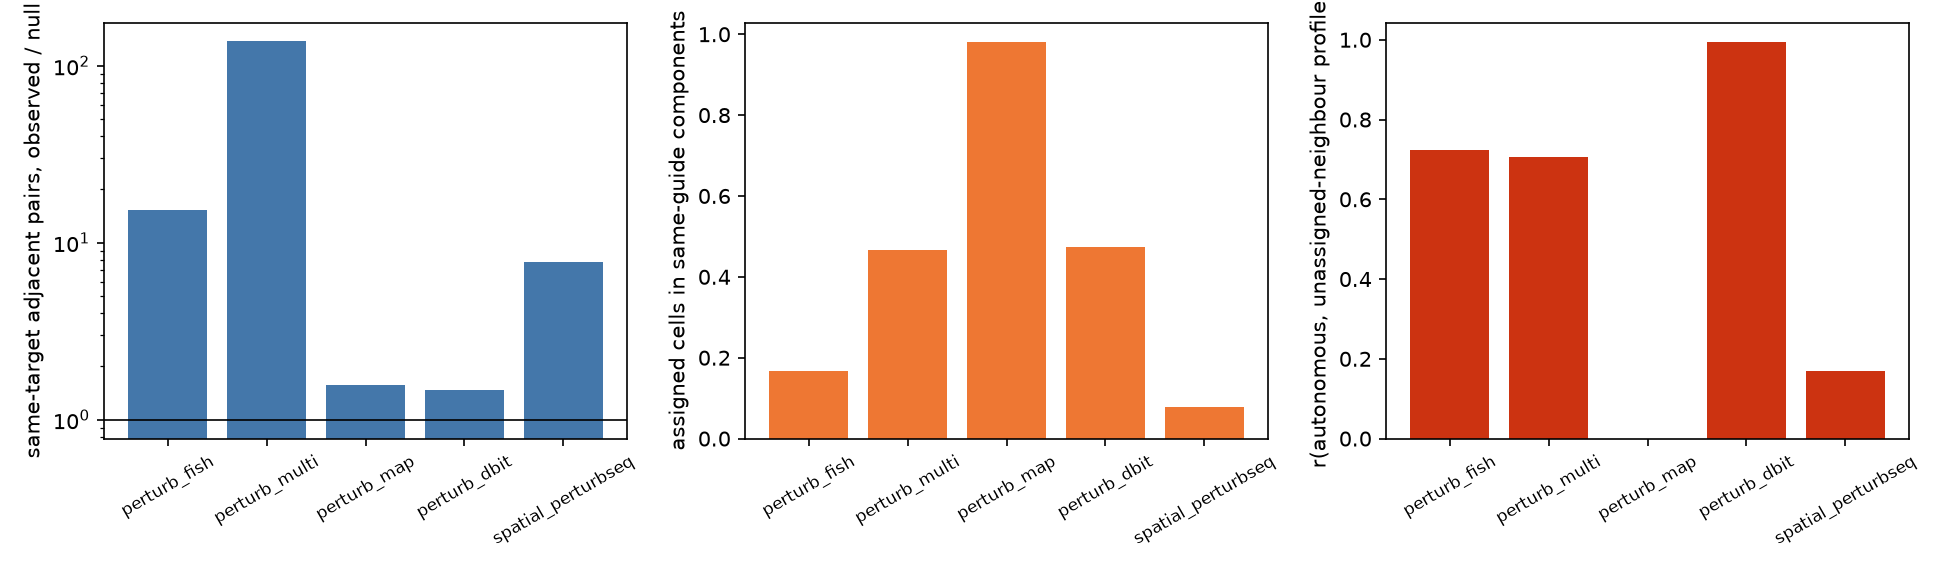
\includegraphics[width=\textwidth]{figures/fig1_clonality.png}
\caption{Same-guide clustering across datasets. Left: observed over expected same-target
adjacent pairs on the pruned Delaunay graph (log scale). Middle: fraction of guide-assigned
cells in same-guide connected components of size two or more. Right: median correlation
between a target's autonomous profile and the profile of unassigned cells adjacent to it.
Source: \texttt{reports/audit/*/clonality.json}.}
\label{fig:clonality}
\end{figure}

\subsection{Global permutation nulls are anticonservative; a spatial basis restores calibration}
Figure~\ref{fig:calib} shows the non-targeting calibration of each estimator configuration on
the two single-cell MERFISH datasets. The stratified difference in means (E1) with strata
sample $\times$ cell type and a studentized permutation null gives \FishNtcPRingZero{} of
first-ring NTC tests at $p<0.05$ in Perturb-FISH and \MultiNtcPAuto{} of autonomous NTC
tests in Perturb-Multi. The mechanism is spatial autocorrelation of expression: the few
recipients exposed to a given target sit around one clone and share its niche, while the
permutation null compares them with NTC cells anywhere in the section. Spatial tiles as
strata restore calibration (2.5 to 3.8\% at $p<0.05$ at 150 to 400~$\mu$m) at the cost of
almost all identified tests, including the autonomous ones: in a clonal tumour screen the
"autonomous" contrast of a clone against distant control cells is as confounded by niche as
the spillover contrast. Regression adjustment (E2) with a per-sample Gaussian radial basis of
40 centres as the spatial random effect keeps positivity. On Perturb-FISH its NTC pseudo-target
rates at $p<0.05$ are \FishNtcPAuto{} (autonomous), \FishNtcPRingOne{} (15 to 30~$\mu$m) and
\FishNtcPRingTwo{} (30 to 60~$\mu$m) but \FishNtcPRingZero{} in the first ring, and on the
simulator the same configuration fails the pre-registered gate under clonal assignment
(Section~\ref{sec:bench}): identifying the ring coefficients from recipients only (amendment
A5), clustering standard errors by spatial tile (A6) and replacing the analytic test by the
stratified permutation null (A7) each changed the picture without bringing the outer rings
below the 0.08 ceiling (0.14 to 0.29). On Perturb-Multi the basis leaves the spillover rings at
\MultiNtcPRingOne{} and \MultiNtcPRingTwo{} (autonomous \MultiNtcPAuto). E2 is therefore an
exploratory estimator in this paper: its counts are shown with the NTC-scaled expectation and
the implied false discovery proportion, never alone.

\begin{figure}[t]
\centering
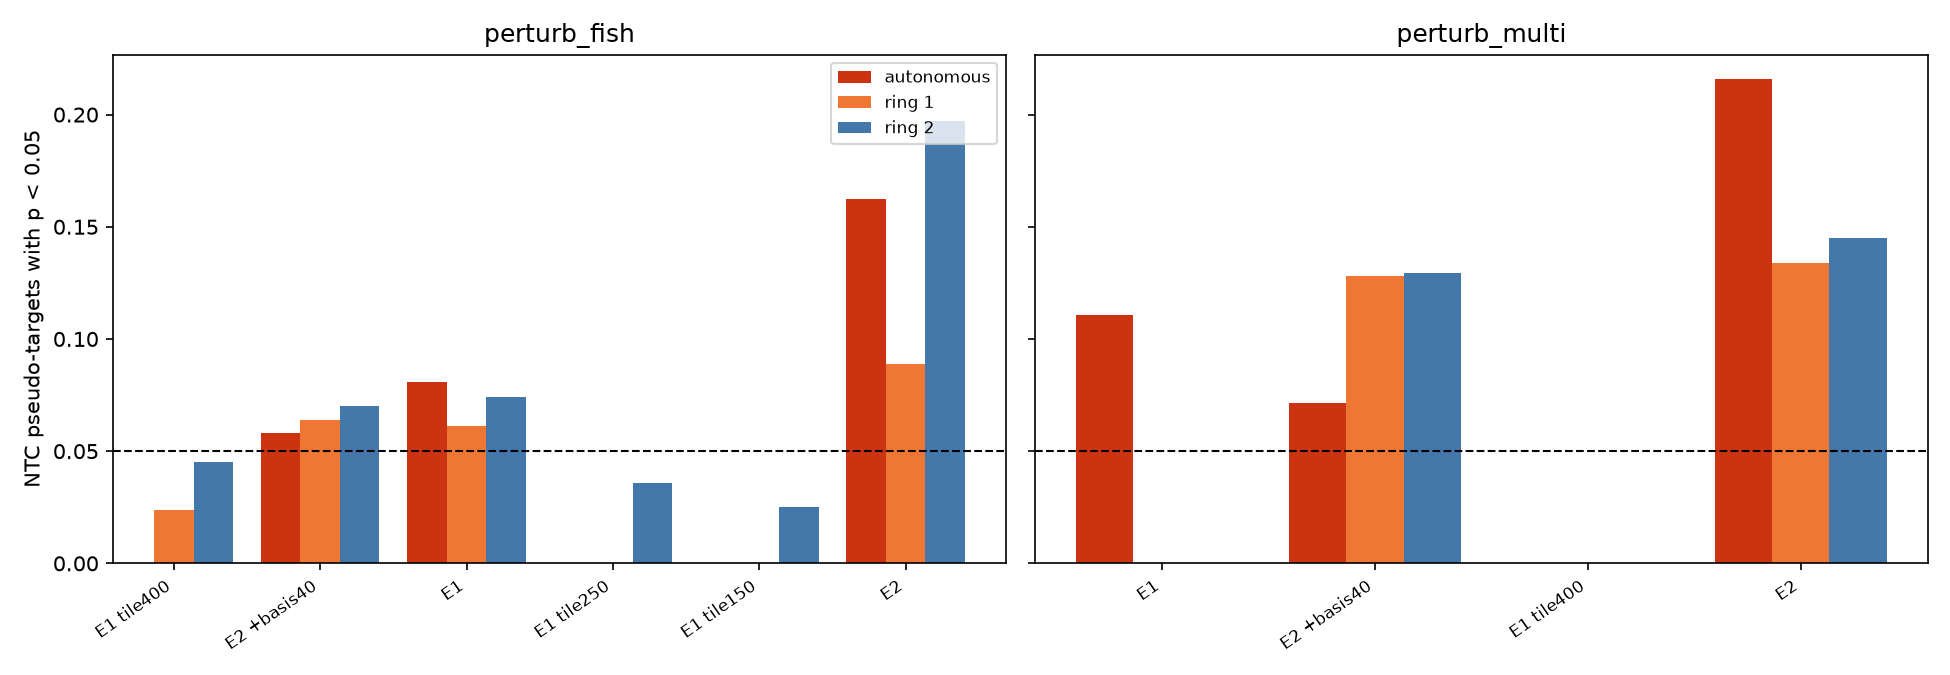
\includegraphics[width=\textwidth]{figures/fig2_calibration_real.png}
\caption{Non-targeting calibration on real data. Fraction of NTC pseudo-target tests with
$p<0.05$ for the autonomous contrast and for the two outer rings, per estimator
configuration. Dashed line: nominal 0.05. Source: \texttt{results/summary/real\_data\_calibration.csv}.}
\label{fig:calib}
\end{figure}

\subsection{Simulator benchmark}
\label{sec:bench}
Figure~\ref{fig:bench} and Table~\ref{tab:bench} report, on geometry copied from the
Perturb-FISH tumour section, the NTC false-positive rate, power and false discovery
proportion of the estimators for planted spillover under null, plain, bleed-through,
density, batch, clonal and misassignment scenarios. The neighbour $t$-test (E0, the design of
published analyses) has the highest apparent power and false discovery proportions of 0.27 to
0.59, with 10\% NTC false positives under clonal assignment. E1 and E2 hold NTC false positives
at 4 to 7\% in the outer rings except E1 under clonal assignment; the doubly robust estimator
(E3) is anticonservative in the first ring; the graph neural network (E4) ranks planted
spillover best (AUROC about 0.9 versus 0.6 for E1 and E2 at 10{,}000 cells) but its bootstrap
intervals are not usable for inference (null false-positive rate above 0.9). Normalisation
induces a compositional shift on every gene when a perturbation changes 10 to 20\% of a small
panel; the benchmark truth is corrected for it and the effect is itself a caveat for
panel-based assays.

\begin{table}[t]
\centering
\small
\caption{Simulator benchmark for spillover in the outer rings (mean over rings 1 and 2 and
over replicates): non-targeting false positives at $p<0.05$, power at $q<0.1$, AUROC and false
discovery proportion at $q<0.1$, by scenario and estimator. Source:
\texttt{paper/tables/benchmark\_spillover.tex}.}
\label{tab:bench}
\begin{tabular}{llrrrr}
\toprule
scenario & estimator & NTC FP (p<0.05) & power (q<0.1) & AUROC & FDP (q<0.1) \\
\midrule
everything & E1 & 0.09 & 0.10 & 0.67 & 0.66 \\
everything & E2 & 0.09 & 0.24 & 0.72 & 0.54 \\
everything & E2\_perm & 0.07 & 0.19 & 0.75 & 0.68 \\
everything & E2\_spatial\_perm & 0.08 & 0.16 & 0.76 & 0.84 \\
everything & E3 & 0.10 & 0.16 & 0.59 & 0.76 \\
no\_effect & E1 & 0.06 & -- & -- & 1.00 \\
no\_effect & E2 & 0.05 & -- & -- & 1.00 \\
no\_effect & E2\_perm & 0.04 & -- & -- & 1.00 \\
no\_effect & E2\_spatial\_perm & 0.03 & -- & -- & 1.00 \\
no\_effect & E3 & 0.06 & -- & -- & 1.00 \\
spill & E1 & 0.06 & 0.26 & 0.76 & 0.37 \\
spill & E2 & 0.05 & 0.36 & 0.81 & 0.23 \\
spill & E2\_perm & 0.04 & 0.16 & 0.75 & 0.34 \\
spill & E2\_spatial\_perm & 0.04 & 0.15 & 0.74 & 0.41 \\
spill & E3 & 0.06 & 0.29 & 0.76 & 0.27 \\
spill\_bleed & E1 & 0.05 & 0.43 & 0.84 & 0.22 \\
spill\_bleed & E2 & 0.05 & 0.45 & 0.84 & 0.23 \\
spill\_bleed & E3 & 0.07 & 0.35 & 0.78 & 0.34 \\
spill\_clonal & E1 & 0.09 & 0.10 & 0.64 & 0.72 \\
spill\_clonal & E2 & 0.07 & 0.18 & 0.68 & 0.48 \\
spill\_clonal & E2\_perm & 0.07 & 0.23 & 0.84 & 0.67 \\
spill\_clonal & E2\_spatial\_perm & 0.07 & 0.20 & 0.84 & 0.83 \\
spill\_clonal & E3 & 0.09 & 0.12 & 0.59 & 0.76 \\
spill\_density & E1 & 0.05 & 0.30 & 0.81 & 0.26 \\
spill\_density & E2 & 0.05 & 0.36 & 0.81 & 0.21 \\
spill\_density & E3 & 0.06 & 0.27 & 0.76 & 0.28 \\
spill\_misassign & E1 & 0.05 & 0.51 & 0.85 & 0.22 \\
spill\_misassign & E2 & 0.06 & 0.53 & 0.86 & 0.22 \\
spill\_misassign & E3 & 0.06 & 0.44 & 0.82 & 0.22 \\
\bottomrule
\end{tabular}

\end{table}

\begin{figure}[t]
\centering
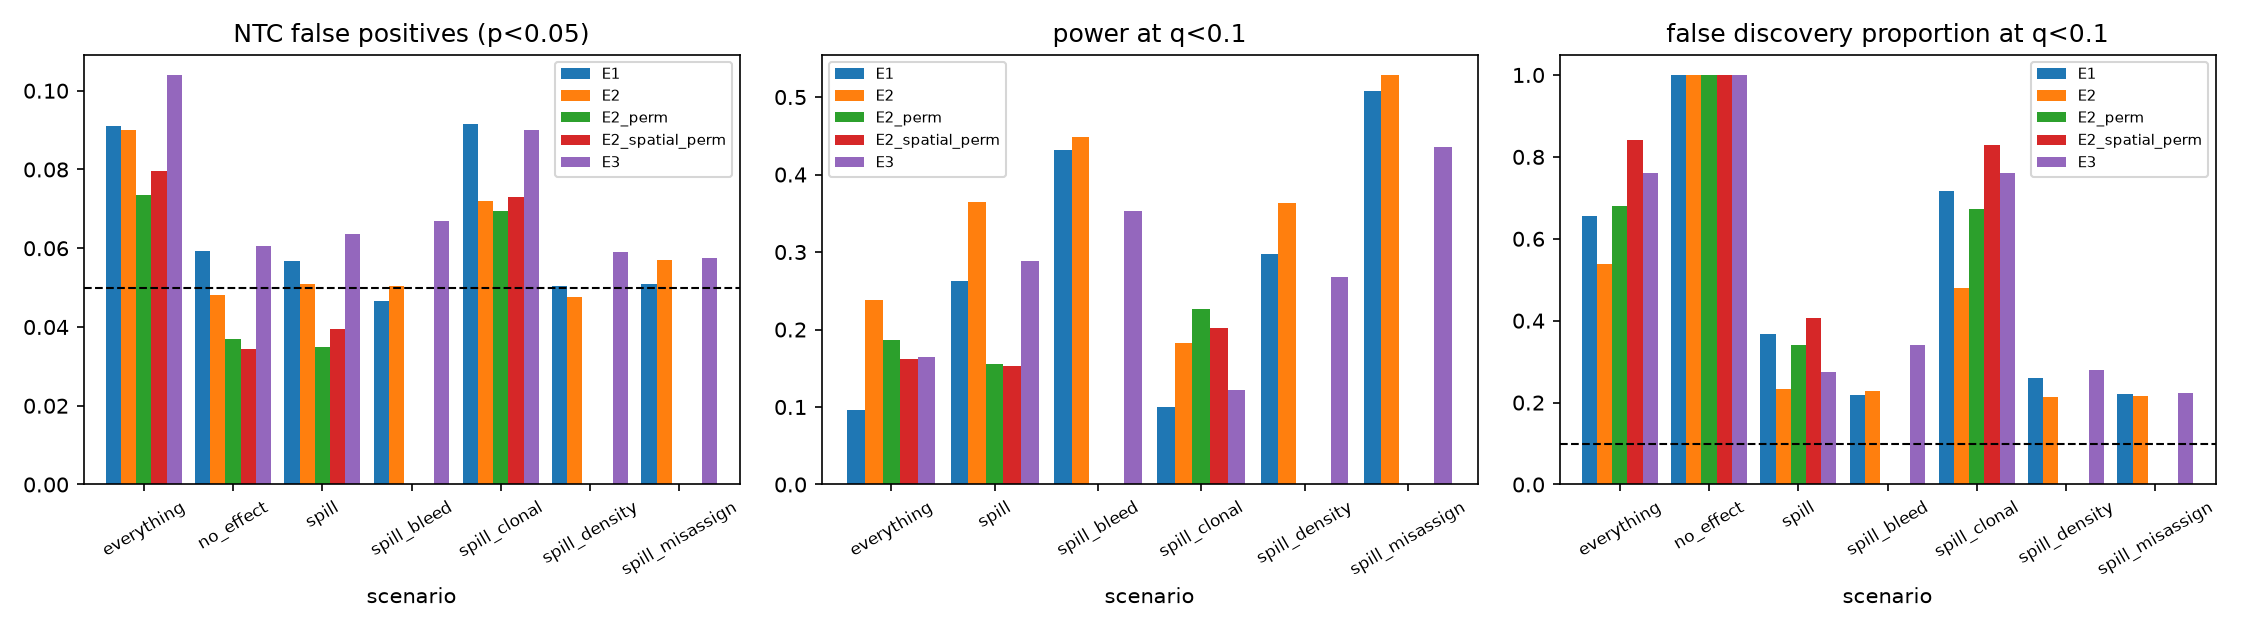
\includegraphics[width=\textwidth]{figures/fig3_benchmark.png}
\caption{Simulator benchmark for spillover in the outer rings: NTC false positives, power at
$q<0.1$ and false discovery proportion, by scenario and estimator. Source:
\texttt{paper/tables/benchmark\_spillover.csv}.}
\label{fig:bench}
\end{figure}

\subsection{What survives in Perturb-FISH, and what does not in Perturb-Multi}
Under the calibrated configuration (E1, 250~$\mu$m tiles, NTC recipients, clean controls),
Perturb-FISH yields \EOneTileAutoHits{} autonomous and \EOneTileSpillHits{} spillover calls at
$q<0.1$ over \EOneTileNTests{} identified tests; the pre-registered hypotheses H2 and H3 are not
supported. Under the exploratory configuration (E2 with spatial basis and the stratified permutation
null), whose non-targeting rates on this dataset are nominal (\FishNtcPAuto{} autonomous,
\FishNtcPRingZero{}, \FishNtcPRingOne{}, \FishNtcPRingTwo{} by ring), the same dataset gives
\FishAutoHits{} autonomous calls over \FishNTests{} tests against a non-targeting expectation of
about 8, and \FishSpillHits{} spillover calls against an expectation of 0 (ring-level numbers in
the notebook). The thousands of calls produced by the same model with analytic standard
errors (notebook entries of 07:47 to 08:03) were products of anticonservative uncertainty,
as their NTC-estimated false discovery proportions of 0.3 to 0.5 had indicated. The bleed-through detector applied to the E2
profiles finds no proportional transfer of the autonomous profile into the first ring
beyond a minor component (variance explained in the first ring minus the last ring:
\FishArtifactFrac; projection coefficient \FishAlphaRingZero{} in the first ring against
0.10 in the last), so segmentation spill of the autonomous programme is detectable but small. Ranking targets by their outer-ring E2 evidence
(Figure~\ref{fig:ranking}), \FishNAboveNtc{} of \FishNRanked{} knockouts exceed the 95th
percentile of NTC pseudo-target scores (\FishNtcScoreQ), led by \FishTopTarget{} (score
\FishTopScore). The list is dominated by TLR4/NF-$\kappa$B adaptors, which is both the expected
biology of a tumour-cell NF-$\kappa$B knockout changing cytokine output and what residual
niche confounding produces; given the gate failure, it is a hypothesis list. In
Perturb-Multi, \MultiSpillHits{} exploratory spillover calls over \MultiNTests{} tests do not
exceed the NTC-scaled expectation (NTC-estimated false discovery proportion \MultiSpillFdp):
no spillover is detectable in the 209-gene liver panel with any configuration tried.

\begin{figure}[t]
\centering
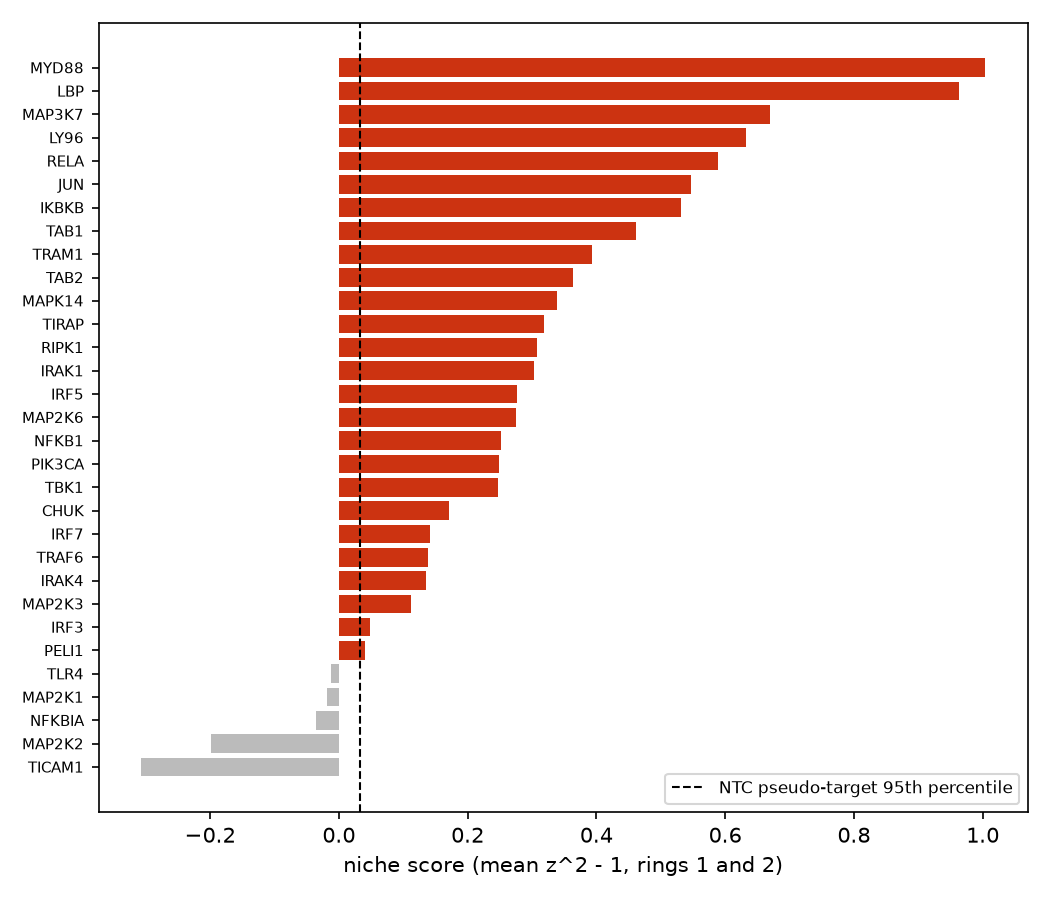
\includegraphics[width=0.7\textwidth]{figures/fig4_ranking.png}
\caption{Niche-remodelling ranking in Perturb-FISH (E2 with spatial basis, rings 15 to
60~$\mu$m). Red: above the 95th percentile of NTC pseudo-target scores (dashed). Source:
\texttt{paper/tables/niche\_ranking\_fish.csv}.}
\label{fig:ranking}
\end{figure}

\subsection{Prediction from gene embeddings fails honestly}
Leave-one-target-out kernel ridge regression from Replogle K562 Perturb-seq embeddings
\citep{replogle2022} or GO embeddings predicts held-out autonomous profiles with mean
$r$ = \FishPredRepAuto{} (permuted-embedding null \FishPredNullRepAuto) and spillover
profiles with \FishPredRepSpill{} (null \FishPredNullRepSpill) in Perturb-FISH, with GO giving
\FishPredGoAuto{} (\FishPredNullGoAuto) and \FishPredGoSpill{} (\FishPredNullGoSpill). A
predictor of niche scores trained on Perturb-FISH and applied to Perturb-Multi through GO
embeddings reaches Spearman \HeldoutRho{} (null \HeldoutNull, empirical $p$ = \HeldoutP) with
\HeldoutOverlap{} overlapping targets. With about thirty targets from one pathway there is
nothing to generalise from, and we report this as the result.

\subsection{Case study and proposed validation}
\label{sec:case}
Figure~\ref{fig:case} shows the top-ranked target. The proposed validation is a two-colour
co-culture or a sorted-neighbour experiment: tumour cells carrying the \FishTopTarget{} guide
mixed at low ratio with barcoded wild-type cells, followed by sorting the wild-type population
by proximity (imaging) or by a contact reporter (synNotch or LIPSTIC-type labelling), and
bulk RNA-seq of contact versus non-contact wild-type cells. The pre-specified readout is the
ring-1 profile of Figure~\ref{fig:case}; the expected outcome under the spillover hypothesis
is a concordant shift of the top ring-1 genes in contact cells only, and under the niche
hypothesis no shift. A conditioned-medium arm separates secreted from contact-dependent
signalling.

\begin{figure}[t]
\centering
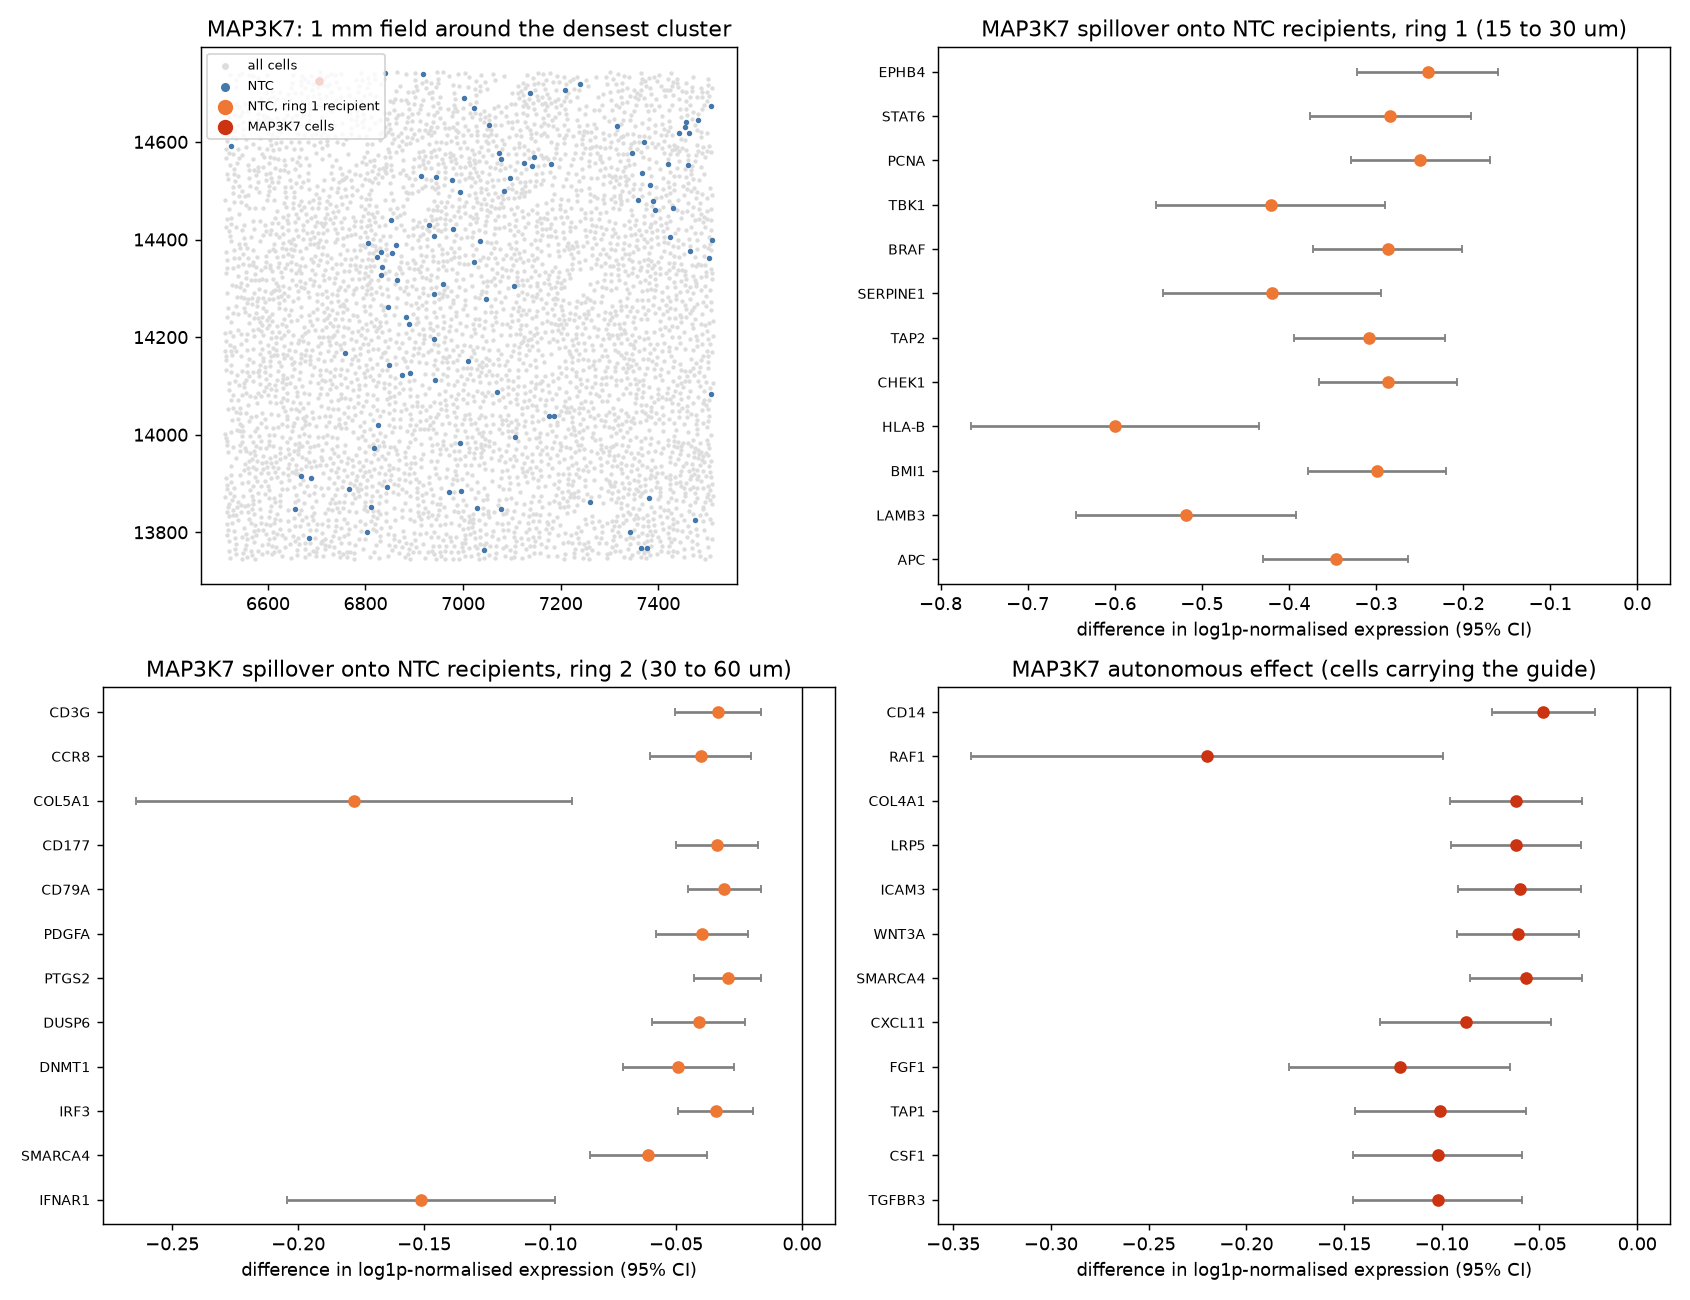
\includegraphics[width=\textwidth]{figures/fig5_case.png}
\caption{Case study of the top-ranked target in Perturb-FISH: spatial field, outer-ring
spillover profiles with 95\% intervals, and the autonomous profile. Source:
\texttt{results/<run>/case\_<target>.png}.}
\label{fig:case}
\end{figure}

\section{Discussion and limitations}
\label{sec:limits}
\begin{itemize}
\item Clonal and delivery-driven clustering of same-guide cells is the first-order structure
of in vivo spatial screens. It invalidates "unassigned neighbour" designs and, through niche
sharing, biases autonomous estimates as well. We handle it by recipient eligibility and a
spatial basis; an explicit undetected-sibling model is future work.
\item No estimator in the ladder is both calibrated and powered under clonal assignment: E1
with local tiles is calibrated and finds nothing; E2 variants keep power and fail the
simulator gate. The first ring (0 to 15~$\mu$m) is anticonservative for every estimator.
We make no spillover claim from these data.
\item BH $q$-values are not nominal under residual confounding; every hit count is reported
with the NTC-scaled expectation and the implied false discovery proportion (0.3 to 0.4 here).
\item The estimators changed after the first real-data runs (amendments A1 to A5 in the
notebook, each declared before its rerun). The discarded results are kept.
\item Pixel-level (Perturb-DBiT) and spot-level (Perturb-map) technologies cannot separate
intra-unit mixing from intercellular effects; their spillover analyses are exploratory.
\item The bleed-through detector only detects proportional transfer of the autonomous profile.
\item E4's uncertainty is not usable; it is reported for ranking only.
\item Prediction from embeddings and transfer across technologies failed; with the target sets
available this is expected and should not be read as evidence against the approach.
\item Edge distance is a bounding-box proxy; tissue masks were not used.
\item Compute constrained Perturb-Multi to five of eleven sections and 150{,}000 cells per
section.
\end{itemize}

\section{Methods}
\label{sec:methods}
\paragraph{Data.} Loaders, accessions, licences and sizes are in \texttt{data/README.md};
counts for Perturb-Multi were recovered exactly from the deposited log-normalised matrix.
\paragraph{Estimands.} See \texttt{docs/estimands.md}; exposure is the vector of ring counts of
$g$-perturbed cells within $D_{\max} = 60~\mu$m (bins 0 to 15, 15 to 30, 30 to 60~$\mu$m).
\paragraph{Estimators.} E0 neighbour $t$-test and pseudobulk DE; E1 stratified difference in
means with a studentized stratified permutation null (200 permutations, permutation-calibrated
$z$, exact permutation $p$ with the Phipson-Smyth correction \citep{phipson2010});
E2 regression adjustment with stratum indicators, own-guide indicator, ring counts for
recipients, centred covariates (local density, log area, edge distance) and a per-sample
Gaussian radial basis, HC1 or cluster-robust standard errors; E3 augmented inverse-probability
weighting with Monte Carlo exposure probabilities \citep{aronow2017}; E4 message-passing GNN
with single-neighbour interventional counterfactuals. BH-FDR \citep{benjamini1995} over all
identified tests per dataset.
\paragraph{Simulator and benchmark.} Negative-binomial counts on real geometry with planted
effects; scoring on null, non-null and composition-shifted pairs; NTC pseudo-targets as exact
nulls.
\paragraph{Reproducibility.} \texttt{make reproduce} regenerates every result from a clean
clone; results are keyed by configuration hash; all DOIs are checked against Crossref.

\bibliographystyle{plainnat}
\bibliography{refs}
\end{document}
